%
% ---- Technologies
%

\section{Conclusion and Future Work}

\begin{shaded}
	
The models are useful for qualitative prediction.  They successfully predicted the non-trivial result that when a shared queue is used in combination with a distributed database, whether or not replication is used, then once the partitions storing the high demand tickets were no longer able to satisfy it, the throughput of the other resources was choked in proportion to the relative demand between them and the skewed resources.  The models also predicted that when using replication, there would also be throughput at the replica node.

However, the models were less successful at quantitative predictions.  When using replication, the throughput was not spread evenly (or randomly) between database nodes, and this also meant that the system was not able to satisfy as much demand as predicted.  This means that it was not possible to use the models to compare which system would make best use of the resources available, as the models suggested - i.e. the models as they stand are not suitable for right-sizing.

The real Cassandra database behaviour is more complex than described by these simple models.  An area of future work might be to adapt these models to make them closer to the true behaviour.  However models tied closely to a particular database implementation are likely to be less universally applicable.

Other areas - different partitioning strategies.

Different queue strategies.  A priority queue for the skewed demand?

An interesting area of future work might be in using the modelling techniques in adaptive algorithms.  A model might be used as a policy for elastic scaling, and compared with the performance of other right-sizing strategies; control theory, machine learning and other model based techniques including statistical.

Data partionining - where the high demand is unknown in advance, we need an adaptive strategy.  Workload-aware clustering algorithms do exist for the placement of new data, e.g. \cite{RN63}, but our use case has a fixed set of tickets.  Re-placement of existing data onto different partitions would be likely to require many reads, writes and deletes.

%
% ---- Operational microservices
%
\subsection{Operational microservices}

A more `natural' microservices architecture partitions the system by operation (Book, Search, Return) with a separate database for each.  The databases maintain eventual consistency via an event streaming application e.g. using Kafka.
\begin{enumerate}
\item Book is an event producer and consumer (produces when a ticket is booked, consumes returned tickets).
\item Search is an event consumer (consumes the state of tickets that are booked and returned).
\item Return is an event producer (produces returned tickets).
\end{enumerate}

\end{shaded}

\begin{figure}
	\caption{Operational microservices architecture}
	\centering
	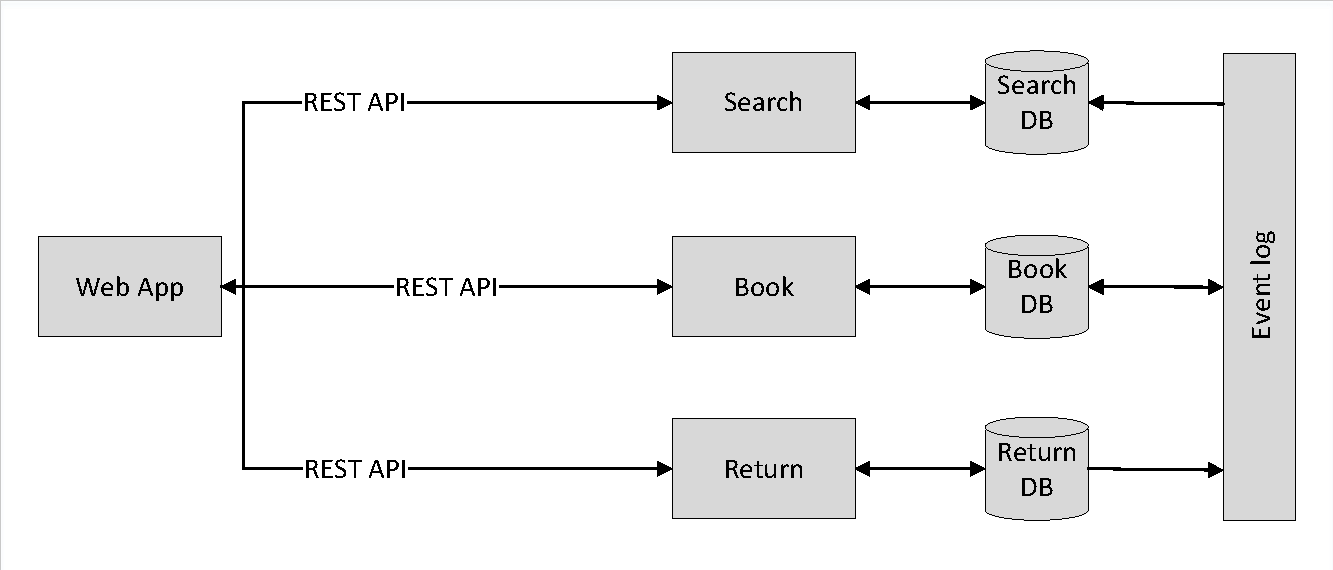
\includegraphics[trim = 5 5 5 5, clip, width=\textwidth]{img/operationmicro}
\end{figure}
